\documentclass{article}

\usepackage[letterpaper]{geometry}
\usepackage{amsmath}
\usepackage{amssymb}
\usepackage{graphicx}

\title{2231 HW 9}
\author{Duncan Wilkie}
\date{3 December 2021}
\begin{document}

\maketitle

\section{}
We may apply Ampere's law to obtain (using cylindrical coordinates' gradient)
\[\nabla \times \vec{B}=\mu_0\vec{J}\Leftrightarrow \vec{J}=\frac{1}{\mu_0}\nabla\times\nabla\times\vec{A}=\frac{1}{\mu_0}\nabla\times\nabla\times(k\hat{\phi})=\frac{1}{\mu_0}\nabla\times\left(\frac{k}{r^2}\hat{z}\right)=\frac{1}{\mu_0}\left( \frac{k}{r^2}\hat{\phi} \right)=\frac{k\hat{\phi}}{{\mu_0r^2}}\]
\section{}
The divergence is, using the fact $B$ is uniform,
\[\nabla\cdot\vec{A}=-\frac{1}{2}\nabla\cdot\left( (r_yB_z-r_zB_y)\hat{i}+(r_zB_x-r_xB_z)\hat{j}+(r_xB_y-r_yB_x)\hat{k}\right)\]
\[=-\frac{1}{2}\left(\frac{\partial r_y}{\partial x}B_z-\frac{\partial r_z}{\partial x}B_y +\frac{\partial r_z}{\partial y}B_x-\frac{\partial r_x}{\partial y}B_z+\frac{\partial r_x}{\partial z}B_y-\frac{\partial r_y}{\partial z}B_x\right)\]
\[=-\frac{1}{2}\left( B_x\left( \frac{\partial r_z}{\partial y}-\frac{\partial r_y}{\partial z} \right)+B_y\left( \frac{\partial r_x}{\partial z}-\frac{\partial r_z}{\partial x} \right)+B_z\left( \frac{\partial r_y}{\partial x}-\frac{\partial r_x}{\partial y} \right) \right)\]
Since $\vec{r}=(x,y,z)$, all the partials are zero, and the divergence is zero. This is consistent with the usual choice of gauge function to make the double curl equal the vector Laplacian.
The curl is, simplifying the above expressions by writing the $\vec{r}$ components explicitly,
\[-2\nabla\times \vec{A}=\nabla\times\left( (yB_z-zB_y)\hat{i}+(zB_x-xB_z)\hat{j}+(xB_y-yB_x)\hat{k}\right)\]
\[=\left( \frac{\partial}{\partial y}\left( xB_y-yB_x \right)-\frac{\partial}{\partial z}\left( zB_x-xB_z \right) \right)\hat{i}\]\[+\left( \frac{\partial}{\partial z}\left( yB_z-zB_y \right)-\frac{\partial}{\partial x}\left( xB_y-yB_x \right) \right)\hat{j}\]\[+\left( \frac{\partial}{\partial x}\left( zB_x-xB_z \right)-\frac{\partial}{\partial y}\left( yB_z-zB_y \right) \right)\hat{k}\]
\[=-2B_x-2B_y-2B_z=-2\vec{B}\]
\[\Rightarrow \nabla\times \vec{A}=\vec{B}\]
Let $\vec{F}=\vec{A}+5\hat{i}$. The gradient and the curl are the same, since there is a partial derivative taken in each case. Yet this is a distinct function. (The theorem that makes this work normally, the Helmholtz theorem, requires $O(r^{-2})$ convergence to zero in the curl and the divergence. The curl is constant here.)

\section*{3a}
Circles within the disk of radius $r$ contain differential line charge $\lambda=\sigma dr$. This charge is moving with speed $v=r\omega$, so the current associated with every circle within the disk is $I=\lambda v=r\omega\sigma dr$. The dipole moment from such a circular current is (presuming the disk lies in the $x$-$y$ plane)
\[\vec{m}_r=I\int d\vec{a}=I\pi r^2\hat{z}=\omega\sigma \pi r^3dr\hat{z}\]
Adding up all the dipole moments of these circles in the disk by an integral, the overall dipole moment is
\[\vec{m}=\int_0^R\omega\sigma\pi r^3dr\hat{z}=\frac{\omega\sigma\pi R^4}{4}\hat{z}\]

\section*{3b}
Similarly to above, we consider circles within the sphere. They have the same dipole moment as above (in both cases, it's just a circle of charge rotating with some angular velocity), but to simplify the integration a change of variables to spherical coordinates must occur, since $r$ in that expression isn't the radial spherical coordinate. Denoting that coordinate by $R$ (since it doesn't change in the integration), by geometric inspection $r=R\sin\varphi$. We also have $dr=Rd\varphi$ from similar inspection, enabling us to compute the total dipole moment as
\[\vec{m}=\int_S\vec{m}_rdr\hat{z}=\int_{0}^{\pi}\omega\sigma\pi R^3\sin^3\varphi Rd\varphi\hat{z}=\frac{4\pi}{3}\omega\sigma R^4\hat{z}\]

\section*{4}
First, we compute the bound surface and volume currents from the magnetization, presuming the magnetization in the $+x$ direction.
\[\vec{J}_b=\nabla\times \vec{M}=0 \textrm{ (uniform)}\]
\[\vec{K}_b=\vec{M}\times \hat{n}=|M|\hat{\varphi}\]
The magnetization at the ends of the cylinder is parallel to the surface, so the bound surface current is zero.
This is exactly the situation of an ideal solenoid: current flows in circles around the surface of an infinitely long cylinder.
Therefore, the magnetic field outside the cylinder is zero, and the magnetic field inside is
\[\vec{B}=\mu_0nI\hat{x}\]
To write this in terms of known quantities, note that $nI$ is the current per length along the cylinder, which is exactly surface current. Therefore, $\vec{B}=\mu_0|K_b|\hat{\varphi}$.
Since $|\vec{K}_b|=|\vec{M}|$, the final expression for the magnetic field is
\[\vec{B}=\begin{cases}
    {\mu_0|\vec{M}|}\hat{x} & \textrm{inside the cylinder} \\
    0 & \textrm{elsewhere}
  \end{cases}\]

\section*{5}
The reasoning about the bound currents from above holds identically here. I.e. the bound volume current is $0$, and the bound surface current is $|\vec{M}|\hat{\phi}$. A (poor) sketch of the magnetic field appears below. The field lines should be symmetric about the axis of the cylinder, and shouldn't have cusps.
\[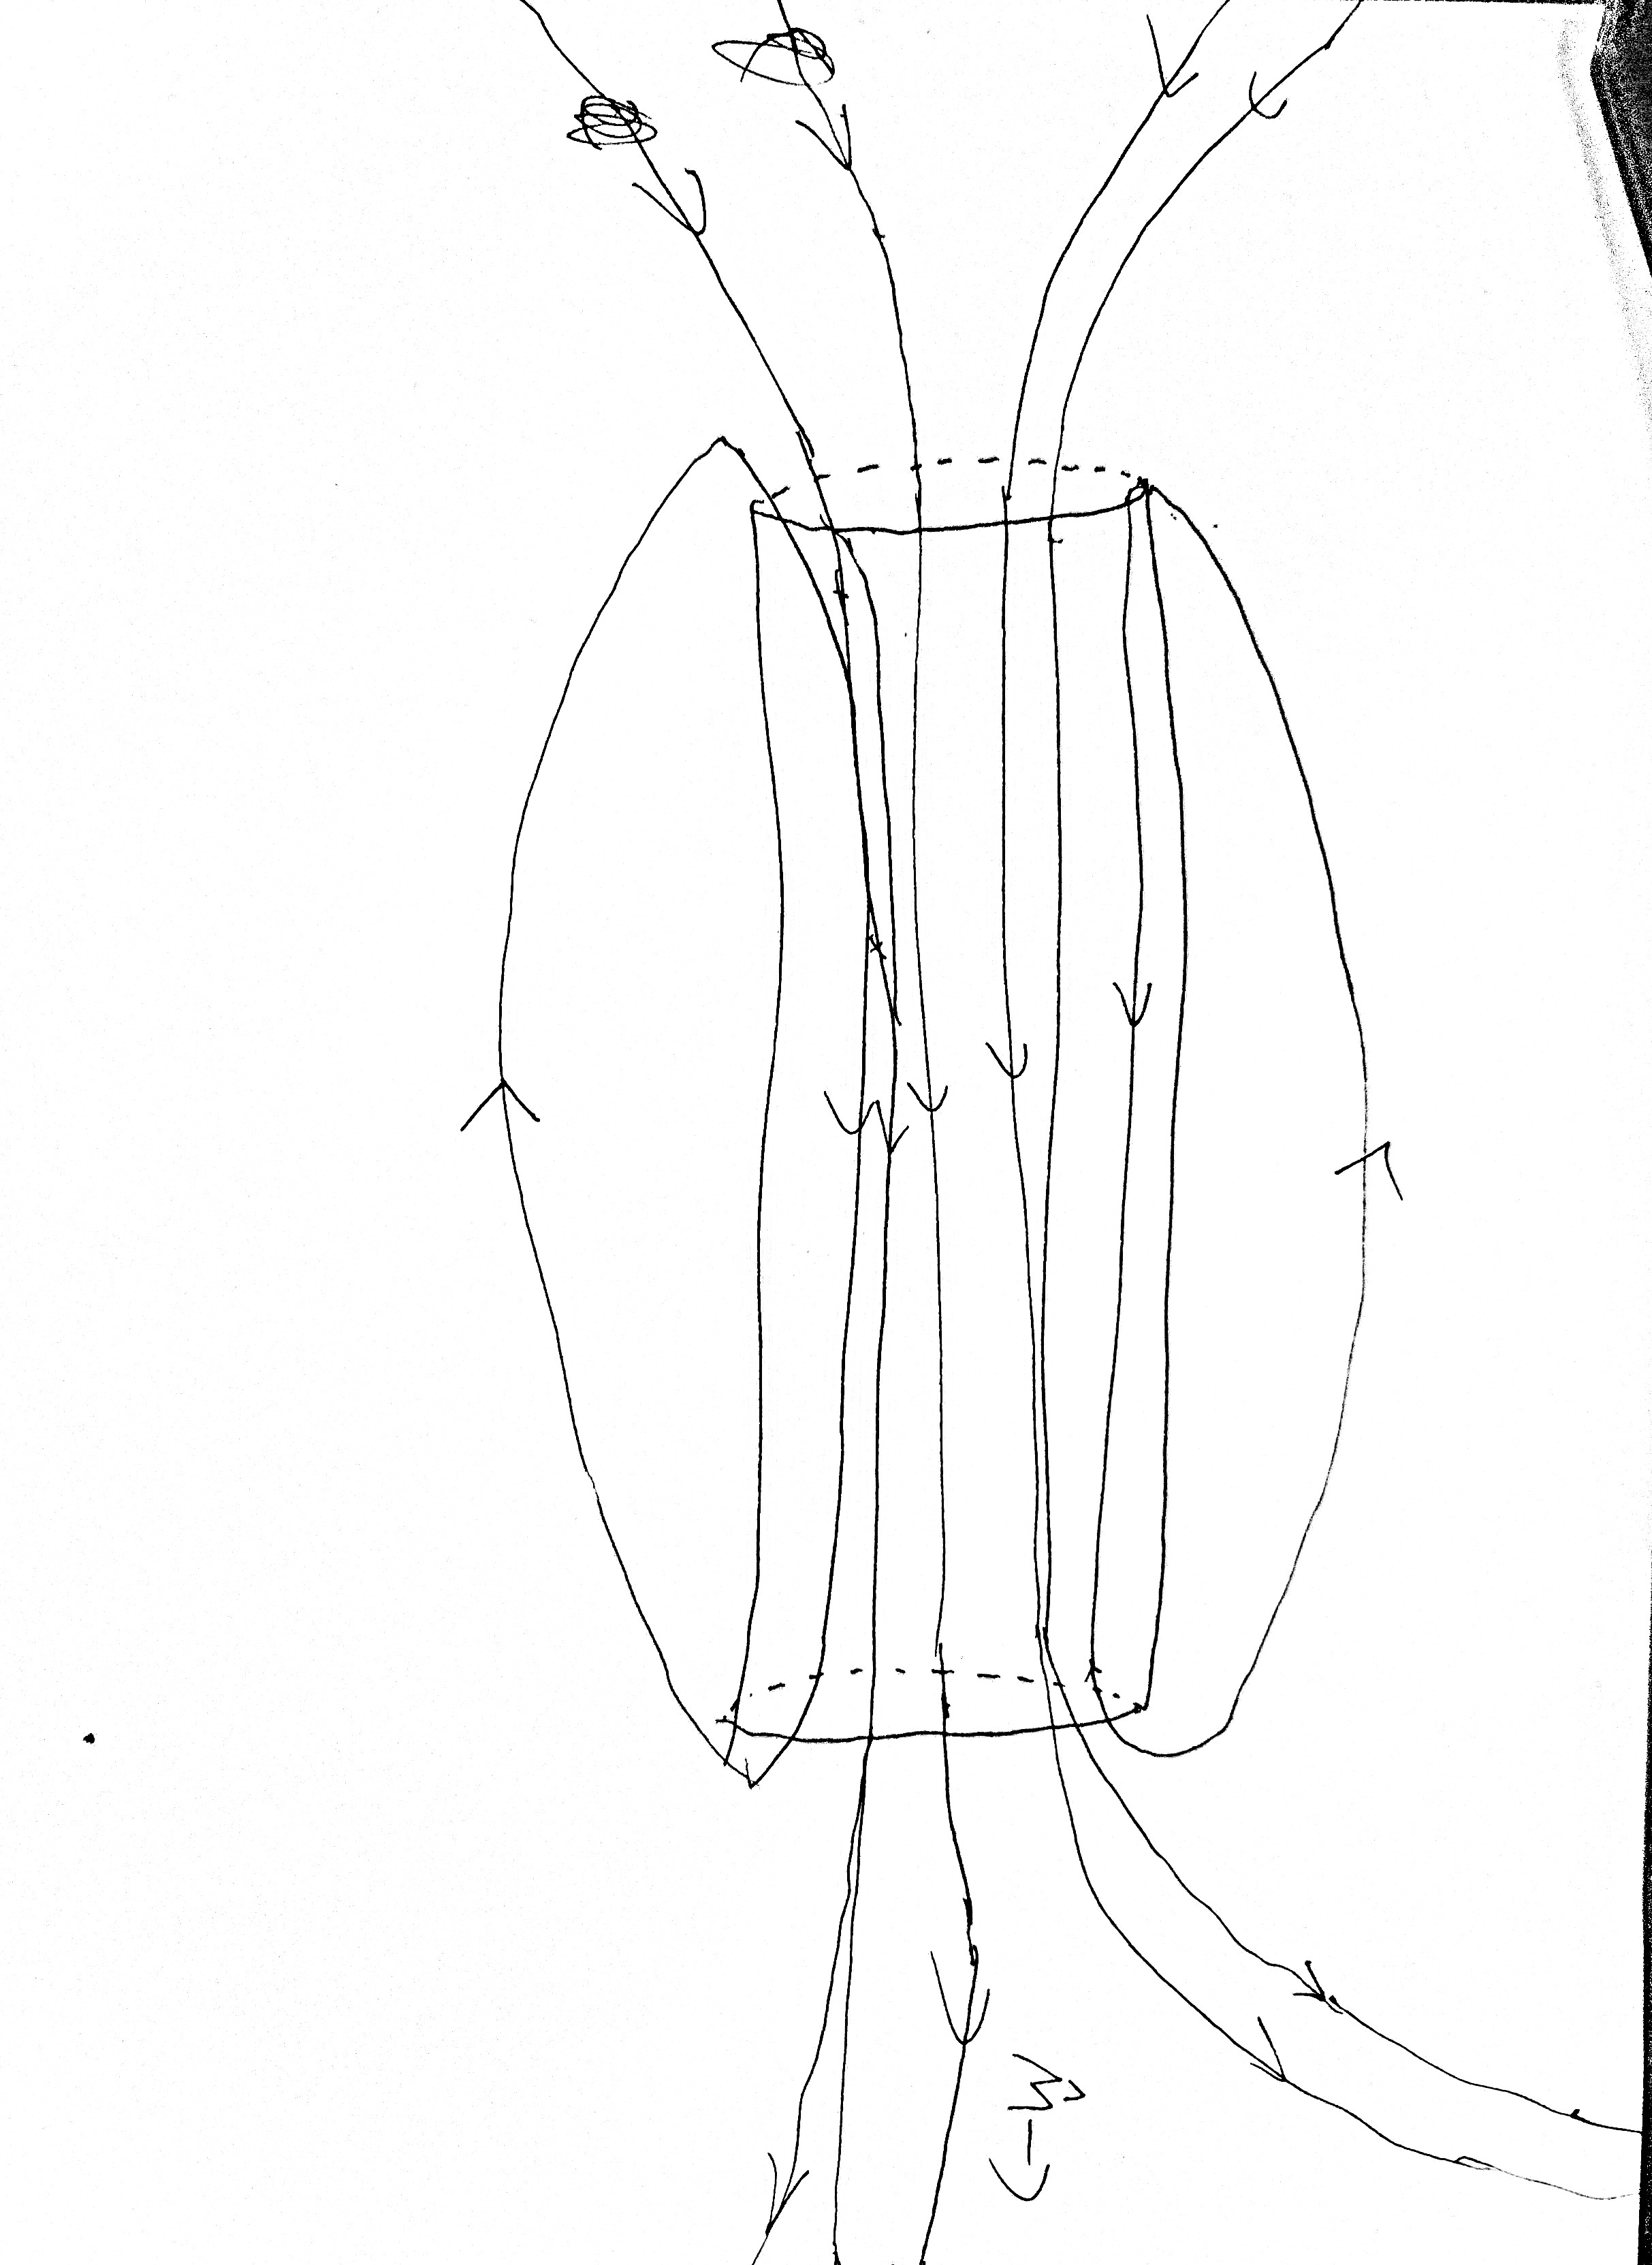
\includegraphics[scale=0.1, angle=90]{img.jpg}\]

\end{document}
%%% Local Variables:
%%% mode: latex
%%% TeX-master: t
%%% End:
